% =====================================================================
%  WACV 2026 — Applications Track — SUPPLEMENTARY MATERIAL
%  Depth carried out of the 8pp main paper (paper_wacv.tex).
%  Compile:  pdflatex supp_wacv && pdflatex supp_wacv
%
%  DOUBLE-BLIND -- see the header of paper_wacv.tex. No \author content, no
%  acknowledgements, no repository URL, no reference to any non-anonymous
%  version of this work, in the body or in comments.
% =====================================================================
\documentclass[10pt,twocolumn,letterpaper]{article}

\usepackage[review,applications]{wacv}
\def\confName{WACV}
\def\confYear{2026}
\def\wacvPaperID{0000}

\usepackage{amsmath,amssymb,amsfonts,bm,mathtools}
\usepackage{amsthm}
\usepackage{graphicx}
\usepackage{booktabs}
\usepackage{multirow}
\usepackage{array}
\usepackage[breaklinks,colorlinks]{hyperref}
\usepackage[capitalize]{cleveref}

\newtheorem{proposition}{Proposition}

% Supplementary numbering: S-prefixed
\renewcommand{\thesection}{S\arabic{section}}
\renewcommand{\thetable}{S\arabic{table}}
\renewcommand{\thefigure}{S\arabic{figure}}

\begin{document}

\title{Supplementary Material\\
\emph{Viewpoint Invariance Is a Theorem, Not a Fit}}
\author{}
\maketitle

This supplement carries the depth condensed out of the main paper: the proof of the invariance theorem
(\cref{sec:supp:proof}), the full invariant-set specification (\cref{sec:supp:cut}), the eight-gate
numerical certificate (\cref{sec:supp:cert}), the complete precision budget (\cref{sec:supp:prec}), the
nondeterminism seed distribution (\cref{sec:supp:seed}), the protocol audit and continuous-time
control (\cref{sec:supp:control}), the units audit behind our comparison against published KIMORE
numbers (\cref{sec:supp:units}), the per-family ablation of the invariant cut
(\cref{sec:supp:ablation}), the in-dataset score-resolution analysis behind the clinical-magnitude
claim (\cref{sec:supp:resolution}), the full second-corpus node-failure curve
(\cref{sec:supp:nodefail}), and the real-camera deployment probe (\cref{sec:supp:realview}). All numbers are reproduced from the same banked artifacts as the main
paper; equation and proposition references (e.g.\ Prop.~1) point to the main text.

% =====================================================================
\section{Proof of the Invariance Theorem}\label{sec:supp:proof}
\begin{proposition}[$SO(3)$-invariance of the read-out; = Prop.~1]
Let the encoder intertwine with the Wigner-$D$ action, so under $g\in SO(3)$ each latent transforms as
$s_j\!\mapsto\! s_j$ (type-$0$) and $v_j\!\mapsto\! D_1(g)\,v_j$ (type-$1$), with $D_1(g)\in SO(3)$
orthogonal and $\det D_1(g)=+1$. Then the projection $\Pi$ (main Eq.~1--2) is invariant under $SO(3)$
for arbitrary encoder weights, and the predicted score is invariant to any rigid camera motion.
\end{proposition}
\begin{proof}
Feeding root-relative coordinates makes every input a difference $\tilde{\bm x}_i-\tilde{\bm x}_j$, so a
camera translation cancels; it remains to treat rotations. Consider each generator of Eq.~1 under
$v\mapsto D_1(g)v$ with $R:=D_1(g)$ orthogonal:
(i) $\tanh s_j$ is a function of a type-$0$ scalar, hence unchanged.
(ii) $\|v_j^c\|=\|Rv_j^c\|$ since $R^{\!\top}R=I$; so $\log(1+\|v\|)$ is invariant.
(iii) $\langle\widehat{Rv},\widehat{Rv'}\rangle=\langle Rv/\|v\|,\,Rv'/\|v'\|\rangle=\langle\hat v,\hat v'\rangle$,
again because $R$ preserves inner products.
(iv) $\det[\widehat{Rv^a},\widehat{Rv^b},\widehat{Rv^c}]=\det(R)\det[\hat v^a,\hat v^b,\hat v^c]=\det[\hat v^a,\hat v^b,\hat v^c]$,
using $\det(R)=+1$; the triple products are invariant under \emph{proper} rotations (and flip sign
under a reflection, $\det=-1$, which is exactly why they narrow the guaranteed group from $O(3)$ to
$SO(3)$). The bone lengths $d_{ij}=\|\tilde{\bm x}_i-\tilde{\bm x}_j\|$ and the anatomical signed volumes
$\chi_\tau$ (normalised determinants of joint triads) are invariant by the same orthogonality and
$\det(R)=+1$ arguments. Finally $\mathrm{mean}_j$ and $\max_j$ are applied identically to invariant
per-joint quantities, hence themselves invariant. Every entry of $\Pi$ is therefore fixed by $g$, for
any weights; the head is a deterministic function of $\Pi$, so the score is invariant. \qed
\end{proof}

% =====================================================================
\section{Full Invariant-Set Specification}\label{sec:supp:cut}
\Cref{tab:invsets} states both generating sets explicitly at the deployed widths ($n_0{=}32$,
$n_1{=}8$; $J{=}25$ joints, $24$ bones, $|\mathcal T|{=}11$ anatomical frames). Both parity classes share
one $\mathrm{mean}\oplus\max$ joint pool; bone lengths and signed volumes are concatenated
index-preserved (unpooled). The parity-even subtotal ($160$) is exactly the projection whose precision
budget is audited in \cref{sec:supp:prec}; the parity-odd completion adds $123$ dimensions.

\begin{table}[t]\centering\footnotesize
\setlength{\tabcolsep}{4pt}
\caption{Structural specification of the invariant cut $\Pi$.}
\label{tab:invsets}
\begin{tabular}{llcc}
\toprule
Generator & Irrep & Count & Dim \\
\midrule
\multicolumn{4}{l}{\emph{Parity-even} --- generating set complete for $O(3)$}\\
\quad scalars $\tanh s$                      & $0e$ & $n_0$            & $32$ \\
\quad vector norms $\log(1{+}\|v\|)$         & $0e$ & $n_1$            & $8$ \\
\quad cosines $\langle\hat v,\hat v'\rangle$ & $0e$ & $\binom{n_1}{2}$ & $28$ \\
\quad\emph{pooled} $\mathrm{mean}\oplus\max$ &      & $2\times68$      & $136$ \\
\quad bone lengths $d_{ij}$                  & $0e$ & per bone         & $24$ \\
\cmidrule(lr){1-4}
\quad\textbf{even subtotal}                  &      &                  & $\mathbf{160}$ \\
\midrule
\multicolumn{4}{l}{\emph{Parity-odd} --- $SO(3)$ chiral completion}\\
\quad triple products $\det[\hat v,\hat v',\hat v'']$ & $0o$ & $\binom{n_1}{3}$ & $56$ \\
\quad\emph{pooled} $\mathrm{mean}\oplus\max$ &      & $2\times56$      & $112$ \\
\quad anatomical volumes $\chi_\tau$         & $0o$ & per frame        & $11$ \\
\cmidrule(lr){1-4}
\quad\textbf{odd subtotal}                   &      &                  & $\mathbf{123}$ \\
\midrule
\quad\textbf{full $SO(3)$ cut}               &      &                  & $\mathbf{283}$ \\
\bottomrule
\end{tabular}
\end{table}

% =====================================================================
\section{Numerical Certificate (E1--E8)}\label{sec:supp:cert}
We certify the \emph{deployed} model. E1--E5 establish that the claimed invariance is present; E6--E8
establish that it is the one we actually have. The three conditions of E3--E4 --- violation at roundoff,
\emph{flat} in angle, and $r\gg1$ --- are what upgrade ``small'' to ``zero'': magnitude alone would not.
Reported figures are from a representative fp64 run; being roundoff-floor quantities they are
\emph{regime}-stable (order of magnitude, sign of slope, $r\!\gg\!10^{5}$) but not bit-reproducible.
\begin{itemize}\itemsep2pt
\item[E1] \textbf{Representation orthogonality:} $\max_g\|\rho(g)^{\!\top}\rho(g)-I\|_F\le10^{-12}$ (fp64).
\item[E2] \textbf{Invariance of the motion channels:} $\delta,\sigma$ verified invariant, not assumed.
\item[E3] \textbf{Rotation sweep:} score violation $\sim\!10^{-16}$ across $\theta\in[0.05,3.0]$~rad, with
log--log slope $|\text{slope}|<0.5$ (flat). A modelling violation grows with angle; roundoff does not.
\item[E4] \textbf{Precision scaling:} $r=\bar\delta^{\mathrm{fp32}}/\bar\delta^{\mathrm{fp64}}
=5.44\times10^{-8}/4.43\times10^{-16}=1.23\times10^{8}$, tracking the machine-epsilon ratio; a genuine
violation would be precision-independent ($r\approx1$).
\item[E5] \textbf{Translation invariance:} on raw world coordinates,
$|s(\bm x{+}\bm c)-s(\bm x)|/|s(\bm x)|=2.6\times10^{-16}$.
\item[E6] \textbf{Parity:} under a reflection the parity-even cut gives \emph{exactly} $0$ (bit-identical
on a mirrored body --- an unintended $O(3)$-invariance), whereas the completed cut gives
$4.4\times10^{-2}$ (seed~0, \texttt{certify\_egru.json}). A single reflection certifies the entire improper coset.
\item[E7] \textbf{Laterality:} permuting left/right joint \emph{indices} (a relabelling, not a
reflection) moves the score by $6.9\times10^{-2}$ / $5.6\times10^{-2}$ for the two cuts (seed~0); both
separate a left- from a right-limb movement. E6--E7 are model-dependent modelling quantities, not
roundoff-floor ones, and vary across seeds.
\item[E8] \textbf{The fix is free:} read-out invariance under Haar-random \emph{proper} rotations (up to
$\theta{=}\pi$), with the parity-odd channels active, is $2.9\times10^{-16}$ --- unchanged. E1--E5 are
likewise over Haar-random $SO(3)$, so the certified invariance is to the full rotation group, of which a
camera azimuth or the NTU cross-view displacement is one instance. We report no separate NTU-specific
invariance measurement: the gates are architectural and the corpus does not change them.
\end{itemize}

% =====================================================================
\section{Complete Precision Budget}\label{sec:supp:prec}
The full fp64$\to$int8 budget --- including the bf16 and int8-activations-only rows --- is reported in
the main paper's deployment table. The int8 cliff is attributable \emph{solely} to activation
grid-rounding: weight-only quantization preserves the theorem (a quantized model is a different
equivariant model), and fp16 is $3.2\times$ tighter than bf16 because equivariance pays in mantissa
bits, which bf16 trades for exponent range.

% =====================================================================
\section{Nondeterminism: Seed Distribution}\label{sec:supp:seed}
The $0.33$~MAD floor quoted in the main paper is the tighter \emph{fixed-configuration} run-to-run
component (init held constant, atomic nondeterminism only). \Cref{tab:seed} gives the wider
\emph{seed-to-seed} distribution (SO(3) EGRU clean MAD per fold across three initializations): mean
across-seed std $0.48$, worst pairwise gap $1.30$. Both exceed every model-vs-model clean gap in the
main accuracy table, so those gaps are ties. cuDNN-deterministic modes remove the cuDNN-GRU atomic
component but not the initialization variance; the structural degradation columns are weight-independent
(Prop.~1 holds for arbitrary weights), so the flat viewpoint curve stayed exactly flat across every seed
while absolute MAD moved.

\begin{table}[t]\centering\small
\caption{Per-(seed,fold) clean MAD, SO(3) EGRU. No retraining beyond the three seeds.}
\label{tab:seed}
\begin{tabular}{cccccc}
\toprule
fold & seed 0 & seed 1 & seed 2 & std & gap \\
\midrule
0 & $7.120$ & $6.778$ & $6.737$ & $0.210$ & $0.383$ \\
1 & $6.680$ & $6.124$ & $5.804$ & $0.443$ & $0.876$ \\
2 & $6.976$ & $7.345$ & $6.623$ & $0.361$ & $0.722$ \\
3 & $6.762$ & $7.363$ & $6.093$ & $0.635$ & $1.270$ \\
4 & $6.469$ & $7.714$ & $6.415$ & $0.735$ & $1.299$ \\
\midrule
\multicolumn{4}{l}{mean across-seed std} & $\mathbf{0.48}$ & \\
\bottomrule
\end{tabular}
\end{table}

% =====================================================================
\section{Protocol Audit and Continuous-Time Control}\label{sec:supp:control}
\textbf{Protocol audit.} The single-exercise audit of the reference point-cloud transformer ---
selection bias $+1.2\pm0.4$~MAD ($18.6\%$ over three seeds), paired subject-cluster bootstrap
$\Delta=-0.44$ (per-seed $[-1.07,+0.20]$, clearing zero in only one of three seeds) --- is reported
per-seed in the main paper. It is \emph{not} subject leakage
(each subject contributes one recording on that slice, so a random split is already subject-disjoint);
the slice simply carries no robust subject-level signal, so we pool the five exercises and gate every
experiment on a per-exercise mean-predictor floor. Pooled, every model clears that floor with its
bootstrap interval entirely below zero, so the fragility is a property of the slice and not of any
architecture evaluated on it.

\textbf{Continuous-time control.} We implement the Neural CDE variant and certify it to the same E1--E8
standard; it satisfies an exact equivariance certificate and \emph{fails} its own measured floor
($8.43$ vs.\ $8.25$ MAD), the cleanest demonstration that a structural guarantee is worthless without
measured signal.
Analysing the adaptive solver, a Dormand--Prince controller accepts/rejects steps on a per-component
scaled-RMS norm that is \emph{not} group-invariant even when the vector field is exactly equivariant, so
rotated and unrotated integrations receive different step grids and de-align; a per-irrep-normalised norm
removes this, driving grid divergence to identically zero.

\textbf{Irregular-sampling null (derived).} A model-free spectral census finds $97.7\%$ of KIMORE's
\emph{positional} energy below the fixed-grid resampling corner (though $70\%$ of \emph{velocity}
energy lies above it), so resampling preserves pose geometry while low-passing the derivative band and
acts as a denoiser on healthy-form exercises, where the discriminative signal is positional --- the null
was predictable before the experiment, though the boundary would move for tremor-dominated tasks. The
mechanism is nonetheless
real: a physiologically calibrated $5$~Hz tremor is recovered from the true irregular stamps at
$r{=}1.000$ under drop rates up to $70\%$, while a resampled estimator decays to $0.785$.

% =====================================================================
\section{Units of the Published KIMORE Numbers}\label{sec:supp:units}
The main text compares our MAD against published KIMORE MAD directly. That is only legitimate if both
are in clinical-score units, and none of those papers states the scale. The question is not academic:
the reference point-cloud transformer standardises its targets with a \texttt{StandardScaler}
($\sigma\!=\!8.466$ on \texttt{Kimore\_ex1}) and its per-epoch training print is in standardised units
while its evaluator inverse-transforms, so the two readings of the same headline number differ by
$8.5\times$.

The published tables settle it without recourse to anyone's source code. Every method in this lineage
reports MAD and MAPE for the same run, with $\mathrm{MAPE}=100\cdot\mathrm{mean}(|y-\hat y|/|y|)$, so
\begin{equation}
\widehat{|y|}\;=\;100\cdot\mathrm{MAD}/\mathrm{MAPE}
\end{equation}
recovers the magnitude of whatever array was handed to the metric. On raw clinical scores it must land
near KIMORE's per-exercise means; on standardised targets it must land near $\mathrm{mean}|z|\!\approx\!0.8$.

\begin{table}[t]
\centering\small
\setlength{\tabcolsep}{4pt}
\begin{tabular}{lccccc}
\toprule
$\widehat{|y|}=100\,\mathrm{MAD}/\mathrm{MAPE}$ & Ex1 & Ex2 & Ex3 & Ex4 & Ex5 \\
\midrule
Du et al.~2021           & 39.4 & 36.6 & 32.8 & 34.1 & 33.2 \\
Deb et al.~2022          & 41.5 & 60.8 & 51.4 & 42.1 & 39.0 \\
Yao et al.~2023          & 40.2 & 35.1 & 32.5 & 35.5 & 36.1 \\
Mourchid et al.~2023     & 39.5 & 77.3 & 34.3 & 38.1 & 32.8 \\
Zhang et al.~2025        & 41.2 & 51.6 & 38.4 & 42.2 & 35.0 \\
Kuang et al.~2025        & 43.2 & 31.4 & 41.0 & 30.6 & 32.2 \\
Kuang et al.~2026        & 54.5 & 40.1 & 48.3 & 63.4 & 18.8 \\
Point-cloud transf.      & 34.1 & 29.6 & 38.1 & 33.4 & 32.4 \\
\midrule
\textbf{true score mean} & \textbf{40.7} & \textbf{35.6} & \textbf{39.5} & \textbf{35.0} & \textbf{36.4} \\
true $\mathrm{mean}|z|$  & 0.80 & 0.87 & 0.79 & 0.86 & 0.84 \\
\bottomrule
\end{tabular}
\caption{Target magnitude recovered from each paper's own published MAD/MAPE pair, against KIMORE's
true clinical Total Score statistics. Every row lands in the score band ($30$--$63$), none anywhere
near the standardised band ($\approx\!0.8$). Rows reporting no MAPE are omitted.}
\label{tab:supp:units}
\end{table}

\Cref{tab:supp:units} is unambiguous: the median recovered magnitude over all $40$ published cells is
$38.1$ against a true per-exercise mean of $35.0$--$40.7$ (median relative error $10.6\%$), while the
standardised reading is excluded by at least $70\times$ --- it would require these papers to have
printed MAPE values in the tens of percent rather than the $0.17$--$6.0$ they report. The published
KIMORE MAD numbers are therefore in $0$--$50$ clinical-score units, and our $6.3$--$6.7$ is on the same
axis.

The convention is also documented at its source, so the inference above is corroborated rather than
load-bearing. Both papers load KIMORE through descendants of a single \texttt{Data\_Loader}, the one
released with the STGCN-rehab benchmark (Deb et al., IEEE TNSRE 2022); the point-cloud transformer's
copy is near-identical line for line. That release's training script inverse-transforms predictions
\emph{and} targets before computing MAD, RMSE and MAPE, and its released label file holds raw clinical
Total Scores. The reporting convention is therefore fixed upstream of any individual paper, and
\cref{tab:supp:units} confirms it independently, from published numbers alone.
The audit is reproduced by \texttt{src/published\_units\_audit.py}, which gates on all three
conditions.

% =====================================================================
\section{Per-Family Ablation of the Invariant Cut}\label{sec:supp:ablation}
Each family of the invariant cut (\cref{sec:supp:cut}) is zeroed at inference on the deployed chiral
model, dimension preserved and with no retraining, resolving the mechanism to family granularity. The
main paper summarises the result; \cref{tab:supp:ablation} is the full table.

\begin{table}[h]
\centering\small
\setlength{\tabcolsep}{4pt}
\begin{tabular}{lcccc}
\toprule
Family removed & Parity & Clean & $\Delta$Acc & nf lost \\
\midrule
--- (full cut)  & ---  & $6.73$ & ---   & $+3.76$ \\
cosines         & even & $8.56$ & $\mathbf{+1.83}$ & $\mathbf{+7.29}$ \\
triple products & odd  & $9.48$ & $\mathbf{+2.75}$ & $-0.16$ \\
bone lengths    & even & $7.40$ & $+0.67$ & $+2.36$ \\
scalars         & even & $6.98$ & $+0.25$ & $+3.46$ \\
vector norms    & even & $6.89$ & $+0.16$ & $+3.51$ \\
anat.\ volumes  & odd  & $6.93$ & $+0.19$ & $+3.43$ \\
\bottomrule
\end{tabular}
\caption{Per-family ablation of the cut (each family zeroed at inference; 3 seeds $\times$ 5 folds).
$\Delta$Acc below the $0.33$ floor is a tie; ``nf lost'' is worst MAD over $8$ dead joints
(full cut $+3.76$).}
\label{tab:supp:ablation}
\end{table}

% =====================================================================
\section{Score Resolution, and Why Not Clinical Bands}\label{sec:supp:resolution}
The natural way to give the MAD scale an in-dataset meaning is to ask whether a score swing moves a
patient across KIMORE's clinical bands. We do not do this, because KIMORE has no such bands. The five
group labels record how a subject was \emph{recruited}, not what score range they occupy, and on every
one of the five exercises the lowest-scoring control sits below the highest-scoring patient
(\cref{tab:supp:inversion}). Assigning bands to these groups would require inventing the boundaries,
which is the same fabrication we decline elsewhere in this paper.

\begin{table}[h]
\centering\small
\setlength{\tabcolsep}{4pt}
\begin{tabular}{lccc}
\toprule
 & lowest control & highest patient & margin \\
\midrule
Es1 & $34.00$ (NE\_ID10) & $50.00$ (P\_ID3)  & $+16.00$ \\
Es2 & $23.00$ (NE\_ID10) & $50.00$ (B\_ID7)  & $+27.00$ \\
Es3 & $30.00$ (NE\_ID10) & $48.00$ (P\_ID1)  & $+18.00$ \\
Es4 & $26.00$ (NE\_ID11) & $42.33$ (B\_ID6)  & $+16.33$ \\
Es5 & $19.67$ (NE\_ID2)  & $50.00$ (P\_ID6)  & $+30.33$ \\
\bottomrule
\end{tabular}
\caption{Clinical Total Score, control vs.\ patient, per exercise. Every row is inverted, by $16$ to
$30$ points of fifty. The group labels are not score strata.}
\label{tab:supp:inversion}
\end{table}

We therefore measure the swing against the score's \emph{resolution}: how large it is relative to the
differences the score is being asked to express. The between-subject sd of the Total Score is $10.01$
(mean over the five exercises; $10.26$ pooled), so the augmented baseline's mean per-sequence swing of
$3.01$ is $0.30$ sd, its $95$th percentile $8.65$ is $0.86$ sd, and its worst sequence $20.12$ is
$2.01$ sd. The ordinal form of the same statement is \cref{tab:supp:reorder}: a pair of subjects
separated by less than the swing is a pair whose ordering a camera relocation can invert, and ordinal
comparison --- is this patient better than that one, or than they were last week --- is what these
scores are used for.

\begin{table}[h]
\centering\small
\setlength{\tabcolsep}{4pt}
\begin{tabular}{lcccc}
\toprule
\% of subject pairs closer than & $n$ pairs & $3.01$ & $8.65$ & $20.12$ \\
\midrule
all pairs              & $14251$ & $20.2$ & $47.7$ & $83.0$ \\
cross-group only       & $11014$ & $17.4$ & $43.1$ & $80.4$ \\
patient vs.\ control   & $7122$  & $12.8$ & $34.3$ & $74.2$ \\
\bottomrule
\end{tabular}
\caption{Fraction of within-exercise subject pairs whose Total Scores are separated by less than the
augmented baseline's mean ($3.01$), $95$th-percentile ($8.65$) and worst-case ($20.12$) per-sequence
viewpoint swing. These are the pairs the camera can reorder. Pairs are formed within an exercise, since
scores are comparable only across subjects performing the same task.}
\label{tab:supp:reorder}
\end{table}

A third, same-patient comparator avoids between-subject variation entirely. Each subject is rated on
five exercises, and the median spread of a subject's own five scores is $4.97$ sd ($12.00$ range). The
swing's $95$th percentile is $1.74\times$ that median within-subject sd and its worst case $4.05\times$,
so at the tail a camera relocation perturbs the score by several times the variation a single patient
already exhibits. This is a conservative yardstick: different exercises are different measurements, so
the within-subject spread is an upper bound on within-subject noise, which makes the ratio a lower
bound on the swing's severity.

\textbf{Scope and census.} This measures score \emph{resolution}, not group \emph{discriminability} ---
the claim is that a camera move perturbs the clinical output by an amount comparable to the differences
that output expresses, not that the score classifies pathology, which \cref{tab:supp:inversion} shows it
does not. The analysis uses the $380$ subject--exercise cells present in the released data ($77$
subjects; $5$ of the nominal $385$ cells are absent upstream). Five subjects (B\_ID3, B\_ID4, P\_ID10,
S\_ID5, S\_ID6) carry scores that are not multiples of $1/3$, unlike every other subject's rater
averages; excluding them moves nothing material (mean swing $0.30$ sd, $21.3\%$ of pairs reorderable at
$3.01$), and both readings are emitted by \texttt{src/clinical\_resolution.py}. The swing values are
read from the banked Block-3 aggregate rather than recomputed, so this analysis cannot drift from the
numbers quoted in the main text.

% =====================================================================
\section{Node-Failure Curve and Which Spread We Quote}\label{sec:supp:nodefail}
The main paper summarises second-corpus node failure with one number, AUROC lost from $k{=}0$ to
$k{=}8$ frozen joints. That scalar hides the shape, and the shape is not uniformly in our favour.

\begin{table}[h]
\centering\small
\setlength{\tabcolsep}{5pt}
\begin{tabular}{lccccc}
\toprule
REHAB24-6, AUROC at $k$ frozen joints & $k{=}0$ & $k{=}1$ & $k{=}2$ & $k{=}4$ & $k{=}8$ \\
\midrule
EGRU (ours)    & $0.738$ & $0.714$ & $0.694$ & $0.659$ & $0.602$ \\
PCT (baseline) & $0.707$ & $0.697$ & $0.685$ & $0.660$ & $0.623$ \\
\bottomrule
\end{tabular}
\caption{The full curve behind the single ``AUROC lost'' figure. Mean over $3$ seeds $\times$ $5$
subject-disjoint folds.}
\label{tab:supp:nfcurve}
\end{table}

\Cref{tab:supp:nfcurve} shows the two models \emph{cross} between $k{=}2$ and $k{=}4$: we start
$0.031$ ahead, are level at $k{=}4$ ($0.659$ vs.\ $0.660$), and are $0.021$ behind at $k{=}8$. This is
the same Pareto picture the main paper states for KIMORE --- the point-cloud transformer is the more
node-robust model, and our claim is a trade, not a dominance. Reporting only the endpoint difference
would have made the trade look like a loss on one axis rather than a crossover with a locatable knee.

\textbf{Which spread the $\pm$ denotes.} These runs admit two variances that differ by roughly $5\times$,
and they answer different questions. The \emph{fold-level} sd --- the spread of $5$ subject-disjoint
folds within one seed --- is $0.060$ (EGRU) and $0.065$ (PCT); a fold holds out $2$ of $10$ subjects, so
this is large by construction. The \emph{seed-level} sd --- the spread of the $3$ per-seed means --- is
$0.010$ and $0.023$, because averaging five folds cancels most of the subject variation. The
$\pm$ quoted in the main paper is the seed-level one: it describes \emph{seed reproducibility}, not
confidence in the AUROC given this subject pool. At $10$ subjects the fold-level figure is the honest
guide to how far these numbers would move on a different cohort, which is why this corpus is presented
as a structural replication and not as an accuracy benchmark. Both are regenerated by
\texttt{src/second\_corpus\_tables.py}.

% =====================================================================
\section{A Real Camera Move}\label{sec:supp:realview}
The viewpoint experiment of the main paper applies a rigid rotation to ground-truth Kinect
skeletons. That isolates the geometric effect of viewpoint --- which is what the theorem is about ---
but it holds the sensor fixed, so it cannot see a pose estimator degrading at oblique angles. This
section reports the complementary measurement: the camera is physically moved and the entire
deployed pipeline runs end-to-end.

\textbf{Scope, stated first.} \emph{One} subject and \emph{one} exercise (KIMORE Es1 arm lift). This
is a deployment probe, not a benchmark, and it is reported as such for the same reason the second
corpus is: invariance is a per-prediction structural property, so it is legible at $n{=}1$ where an
accuracy claim would not be. The sensor is a commodity webcam with MediaPipe Pose, not Kinect depth,
so both models are off-distribution and their absolute scores read low ($17.7$ and $35.0$ of fifty).
We therefore report score \emph{shift} relative to each model's own straight-on score and never an
accuracy; the domain gap cancels in a within-model difference and would not cancel in a level.

\textbf{Protocol.} A single $15$~s clip is replayed on a monitor and filmed from seven physical camera
poses --- straight on, $\pm30^\circ$ azimuth, tilted up, tilted down, closer, farther --- giving seven
real captures of the same motion. Frames are mapped to the Kinect-$25$ layout at capture time and
preprocessed by the identical root-relative, median-radius, $t/\tau$ path used for training, then
scored with the paper's own five-fold EGRU and PCT ensembles. No model is retrained or adapted.

\textbf{Why the takes must be phase-aligned.} The clip loops and each recording starts at an arbitrary
point in it, so two takes generally show \emph{different parts of the exercise}. That confound is not
small: scoring windows at different phases of a single fixed-camera take moves our score by an sd of
$1.99$ of fifty, which alone exceeds every cross-viewpoint shift we are trying to measure (PCT, whose
architecture resamples onto a fixed grid and so discards duration, has a much smaller phase
sensitivity of $0.74$). We therefore recover each take's lag by cross-correlating a
\emph{rotation-invariant} descriptor of the motion --- norms and distances only, the same invariant
class as the read-out --- and compare all seven takes on the same motion segment. Aligning on an
invariant signal is what keeps this from begging the question: the alignment cannot itself encode the
camera pose under test. Alignment quality is moderate (per-take $r$ between $0.52$ and $0.61$), which
is why the conclusion is checked against lag error below rather than taken on trust.

\begin{table}[h]
\centering\small
\setlength{\tabcolsep}{5pt}
\begin{tabular}{lcc}
\toprule
Camera pose & EGRU (ours) & PCT \\
\midrule
$-30^\circ$ azimuth & $-0.59 \pm 0.19$ & $+1.89 \pm 0.18$ \\
$+30^\circ$ azimuth & $+0.99 \pm 0.25$ & $-2.36 \pm 0.13$ \\
tilt up             & $-0.49 \pm 0.22$ & $-2.56 \pm 0.16$ \\
tilt down           & $+0.38 \pm 0.23$ & $-1.26 \pm 0.12$ \\
closer              & $-0.55 \pm 0.22$ & $-3.25 \pm 0.13$ \\
farther             & $-1.41 \pm 0.19$ & $-1.62 \pm 0.14$ \\
\midrule
mean $|$shift$|$    & $\mathbf{0.74}$  & $2.16$ \\
worst pose          & $\mathbf{1.41}$  & $3.25$ \\
\bottomrule
\end{tabular}
\caption{Score shift (of fifty) versus the straight-on take, paired over $8$ motion phases in an
$8.8$~s window; $\pm$ is the standard error over those phases. Shifts, not levels: the two models sit
at different absolute scores under this domain shift, so only each column's movement is meaningful.}
\label{tab:supp:realview}
\end{table}

\textbf{Result.} \Cref{tab:supp:realview} and \cref{fig:supp:realview}: our score moves $0.74$ of fifty
on average across the six relocations against PCT's $2.16$, a $2.9\times$ gap, and our \emph{worst}
pose ($1.41$) is still smaller than PCT's shift at five of the six poses. Both models move by amounts
that are resolvable against the paired standard error --- five of six poses for ours, six of six for
PCT --- so this is a smaller effect, not an absent one, and we do not claim otherwise. That is the
expected reading of the theorem rather than an exception to it: Prop.~1 removes the geometric
component of a camera move exactly, and what remains is the pose estimator seeing a different body
from a different angle, which no property of the read-out can undo. The measurement here is how much
of the total sensitivity that geometric component was worth end-to-end.

\textbf{Robustness.} The gap is not an artefact of the two choices it depends on. Perturbing every
recovered lag by $\pm0.5$~s gives ratios of $2.43\times$ and $2.27\times$; equalising control-point
count across takes --- the straight-on reference was captured at $11.7$~fps with real dropped frames
while the others ran at $30$~fps --- gives $2.02\times$. The ordering never inverts, and the
unaligned arms agree in direction ($0.78$ vs.\ $1.65$ at full length, $1.05$ vs.\ $2.00$ at matched
duration). The conservative statement is that PCT's score moves at least twice as far as ours when the
camera is physically relocated. Regenerated by \texttt{src/real\_viewpoint\_probe.py}, which records
the checkpoint SHA-$256$s it loaded in its output artifact.

\begin{figure}[h]\centering
  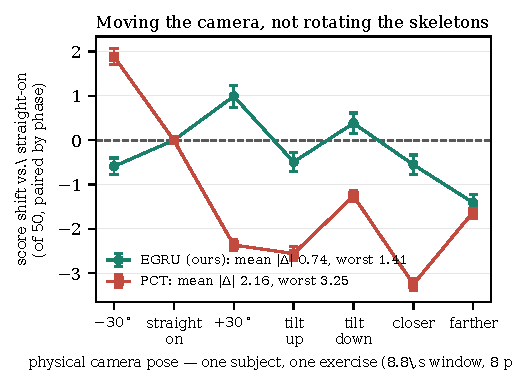
\includegraphics[width=\linewidth]{fig_realview}
  \caption{Paired score shift across seven physical camera poses, one subject and one exercise, each
  model relative to its own straight-on score. Error bars are the standard error over $8$ motion
  phases. This measures shift, not accuracy.}
  \label{fig:supp:realview}
\end{figure}

\end{document}
